\documentclass[12pt]{report}

\usepackage[utf8]{inputenc}
\usepackage{stmaryrd}
\usepackage[french]{babel}
\usepackage{amsmath}
\usepackage{graphicx}
\usepackage{subcaption}
\usepackage{color}
\usepackage{amsfonts}
\usepackage{amssymb}
\usepackage{bm}
\usepackage{hyperref}

\title{Résolution de l'équation de précession d'un moment magnétique par réseau de neurones}

\author{
  Matthieu Carreau\\
  Telecom Paris, Institut Polytechnique de Paris\\
  F-91120, Palaiseau, France\\
  \texttt{matthieu.carreau@telecom-paris.fr} \\
  [1em] Supervisors: \\
  Stam Nicolis\\
  Institut Denis Poisson\\
  Université de Tours, Université d'Orléans, CNRS (UMR7013)\\
  Parc de Grandmont, F-37200, Tours, France\\
  \texttt{stam.nicolis@lmpt.univ-tours.fr}\\
  [1em] \\
  Pascal Thibaudeau\\
  CEA Le Ripault\\
  BP 16, F-37260, Monts, France\\
  \texttt{pascal.thibaudeau@cea.fr}
}
\date{Juillet 2022}

\begin{document}

\maketitle

\begin{abstract}
    {\color{red}{Faire un résumé de ce qu'il y a dans ce document}}
\end{abstract}
    
\tableofcontents{}
    
\chapter{Introduction}
\label{Introduction}

Ce rapport est le compte-rendu d'un stage d'un mois ayant pour objet la mise en place et l'implémentation de méthodes de résolution d'équations différentielles à l'aide de réseau de neurones. 
Le problème physique étudié est celui de la précession d'un moment magnétique dans un champ magnétique, que l'on décrira dans un premier temps par l'équation de précession de Larmor~\cite{PrecessionLarmor}, puis par l'équation de Landau-Lifshitz-Gilbert~\cite{EquationGilbert}.
Cette seconde version de l'équation ne possède pas de solution analytique connue, c'est pourquoi il est pertinent de se pencher sur des méthodes numériques pour en obtenir des solutions approchées.

L'approche proposée ici consiste à utiliser des réseaux de neurones, connus pour leur capacité à approcher des fonctions~\cite{FunctionApproximation}, pour trouver des fonctions "proches" d'être solution d'une équation différentielle.
On utilise par conséquent les réseaux de neurones à la manière de ~\cite{MLWithApp}, ~\cite{ANNforOPDEs} et ~\cite{HighOrderHybrid}, en utilisant les algorithmes d'optimisation connus pour minimiser une fonction d'erreur, qui indique dans quelle mesure une fonction candidate, construite à partir du réseau de neurones, est proche d'être solution.

On écrira lorsque cela sera possible l'équation différentielle d'inconnue $\bm{M}: \mathbb{R} \to  \mathbb{R}^n$ (vecteur adimensionné représentant le moment magnétique) sous une forme similaire à la suivante, où $\bm{g}:  \mathbb{R}\times\mathbb{R}^n \to  \mathbb{R}^n$ est une foncion connue :

\begin{equation}
    \left\{
        \begin{aligned}
            \frac{d\bm{M}(t)}{dt} &= \bm{g}(t, \bm{M}(t)) \\
            \bm{M}(0) &= \bm{M}_0
        \end{aligned}
    \right.
\label{eq:equa dif example}
\end{equation}

La méthode consiste ensuite à construire une fonction candidate pour l'équation différentielle comme une somme de deux termes.
le premier est un terme non ajustable vérifiant la condition initiale, et le deuxième dépendant des paramètres à entraîner représentés par le vecteur $\bm{P}$. Ce dernier est construit de façon à ne pas influencer la valeur initiale de la fonction, afin que la condition initiale soit toujours satisfaite, ceci étant réalisé grâce à une fonction $f:\mathcal{R}\to\mathcal{R}$ fixée à l'avance (souvent $f = id_{\mathcal{R}}$)

\begin{equation}
    \bm{\Tilde{M}}(t) = \bm{M}_0 + f(t)\mathcal{N}(t,\bm{P}) 
\label{eq:solution candidate générique}
\end{equation}
    
On définit ensuite une fonction d'erreur, que l'on calcule à partir de $N$ points $(t_i)_{i\in \llbracket 1, N \rrbracket}$ de l'intervalle d'étude, de la forme :

\begin{equation}
    E ({\bm P})= \sum_{i=1}^{N} (\frac{d\bm{\Tilde{M}}}{dt}(t_i) -g(t_i, \bm{\Tilde{M}}(t_i)))^2   
\label{eq:fonction d'erreur générique}
\end{equation}

Il s'agira enfin d'utiliser différentes méthodes d'optimisation propres au réseaux de neurones afin de trouver un vecteur $\bm P$ qui minimise (et idéalement annule) cette fonction d'erreur.

On s'interresera dans le chapitre~\ref{chap:ode_1} à la résolution d'une équation différentielle à une dimension, en choisissant d'abord le terme ajustable $\mathcal{N}(t,\bm{P})$ sous la forme de séries de Fourier, puis comme la sortie d'un réseau de neurones.
On appliquera dans le chapitre~\ref{chap:precession} les mêmes méthodes pour la résolution d'un système de deux équations couplées représentant le mouvement de précession décrit par l'équation de Larmor.
On étudiera ensuite dans le chapitre~\ref{chap:precession_gilbert} l'effet de l'ajout du terme d'amortissement introduit dans l'équation de Landau-Lifshitz-Gilbert, en utilisant les méthodes qui auront été établies dans les premiers chapitres.
Enfin dans la section~\ref{Conclusion}, je discuterai des résultats obtenus et proposerai quelques perspectives.


%%%%%%%%%%%%%%%%%%%%%%%%%%%%%%%%%%%%%%%%%%%%%%%%%%%%%%%%%%%%%%%%%%%%%%%%%%%%%
\chapter{Equation différentielle à une dimension}
\label{chap:ode_1}

On souhaite dans ce chapitre se familiariser avec différentes méthodes sur un cas simple avec une équation différentielle d'ordre 1 en une dimension.

On considère alors $M$, une fonction réelle à une variable satisfaisant l'équation différentielle suivante, où $M_0$ désigne la valeur initiale de la fonction :

\begin{equation}
\left\{
    \begin{aligned}
        \frac{dM(t)}{dt} + \cos(2\pi t) &= 0 \\
        M(0) &= M_0
    \end{aligned}
\right.
\label{eq:equa dif}
\end{equation}

On cherche à tester les méthodes présentées dans la section~\ref{Introduction} sur l'équation~(\ref{eq:equa dif}), pour tout $t\in [t_a=0,t_b=1]$.
L'équation~(\ref{eq:equa dif}) et sa condition initiale donnée en $t=0$, admet une solution analytique unique qui s'écrit
\begin{equation}
    {M}(t) = M_0 - \frac{1}{2\pi}\sin(2\pi t)
    \label{eq:solution analytique}
\end{equation}


Cela nous permettra par la suite d'évaluer nos solutions numériques, en les comparant à cette solution analytique.


%%%%%%%%%%%%%%%%%%%%%%%%%%%%%%%%%%%%%%%%%%%%%%%%%%%%%%%%
\section{Solutions en séries de Fourier}

On cherche des solutions numériques approchées de l'équation~(\ref{eq:equa dif}) sous la forme de séries de Fourier tronquées avec $H$ harmoniques.
On écrit pour cela la solution approchée $\Tilde{M}$ comme la somme de deux termes, le premier $M_0$ constant non ajustable vérifiant la condition initiale, et le deuxième $\mathcal{N}(t,\bm{A})$ dépendant des coefficients $(A_m)_{H\in \llbracket 1,H \rrbracket}$ représentés par le vecteur $\bm{A}$, construit de façon à ne pas influencer la valeur initiale de la fonction.

\begin{equation}
\left\{
    \begin{aligned}
        \Tilde{M}(t) &= M_0 + {\mathcal{N}}(t,\bm{A}) \\
        {\mathcal{N}}(t,\bm{A}) &= \sum_{m=1}^{H} A_m \sin(2\pi m t) 
    \end{aligned}
\right.
\label{eq:solution Fourier}
\end{equation}




On définit une fonction d'erreur pour ces solutions potentielles, à partir de la valeur de la dérivée de $\Tilde{M}$ aux $N$ points suivants : $\forall i \in\llbracket 1,N \rrbracket, t_i = \frac{i-1}{N} $ :



\begin{equation}
    \begin{aligned}
        E &= \frac{1}{2}\sum_{i=1}^{N} (\frac{d\Tilde{M}}{dt}(t_i) +\cos(2\pi t_i))^2   \\
          &= \frac{1}{2}\sum_{i=1}^{N}(\sum_{m=1}^{H} 2\pi m A_m \cos(2\pi m t_i)+\cos(2\pi t_i))^2 
    \end{aligned}
\label{eq:fonction d'erreur}
\end{equation}

On cherche à présent le minimum de $E$ en tant que fonction de $\bm{A}$. Une condition nécessaire sur $\bm{A}$ pour être un antécédent d'un minimum est 
\begin{equation}
    {\forall l \in\llbracket 1,H \rrbracket, \frac{\partial E}{\partial A_l} = 0}
    \label{eq:condition nécessaire A_l}
\end{equation}

Or ces dérivées partielles sont données pour $l \in \llbracket 1,H \rrbracket$ par :

\begin{equation}
    \frac{\partial E}{\partial A_l} = 
    \sum_{i=1}^{N}(\sum_{m=1}^{H} 2\pi m A_m \cos(2\pi m t_i)+\cos(2\pi t_i))
    2\pi l \cos(2\pi l t_i)
\label{eq:gradient}
\end{equation}


Les deux méthodes suivantes ont pour objectif de trouver les coefficients $(A_m)_{m\in \llbracket 1,H \rrbracket}$ qui vérifient la condition \ref{eq:condition nécessaire A_l}, et de vérifier que le vecteur de coefficients trouvé correspond bien à la solution analytique, i.e $\forall m \in\llbracket 1,H \rrbracket, A_m = -\frac{1}{2\pi}\delta _1 ^m $.


%%%%%%%%%%%%%%%%%%%%%%%%%%%%%%%%%%%%%%%%%%%%%%%%%%%%%%%%
\subsection{Inversion du système linéaire}

Dans le cas de cette modélisation pour la fonction approchée, la condition \ref{eq:condition nécessaire A_l} correspond à un système linéaire de $H$ équations. 
On peut le représenter en définissant les matrices suivantes :

\begin{equation}
    \mathcal{M} = (r_{m,l})_{(m,l)\in \llbracket 1, H\rrbracket ^2}, 
    \bm{A} = \begin{pmatrix}
                A_1 \\
                A_2 \\
                \vdots \\
                A_H
              \end{pmatrix}, 
    \bm{b} = \begin{pmatrix}
                b_1 \\
                b_2 \\
                \vdots \\
                b_H
              \end{pmatrix}
\label{eq:définition notation}
\end{equation}

\begin{equation}
\forall (m,l) \in \llbracket 1, N\rrbracket ^2,
\left\{
    \begin{aligned}
        r_{m,l} &= 2\pi ml \sum_{i=1}^{N}\cos(2\pi mt_i)\cos(2\pi lt_i) \\
        b_l &= -l\sum_{i=1}^{N}\cos(2\pi t_i)\cos(2\pi lt_i)
    \end{aligned}
\right.
\label{eq:définition coefficients}
\end{equation}

On souhaite alors résoudre le système linéaire en écrivant l'équation matricielle le représentant, c'est-à-dire :

\begin{equation}
    \mathcal{M} \bm{A} = \bm{b} \Leftrightarrow \bm{A} = \mathcal{M}^{-1}\bm{b}
\label{eq:équation matricielle}
\end{equation}

On réalise l'implémentation en python, en instanciant les matrices définies précédemment et à l'aide de la bibliothèque \emph{numpy}. 

On peut constater que la matrice $\mathcal{M}$ n'est pas toujours inversible selon le choix de $H$ et $N$. 
En effet, on peut montrer que c'est nécessairement le cas lorsque $H>N$. Il suffit pour cela d'écrire la matrice $\mathcal{M}$ en fonction de la matrice $\mathcal{A}$ de taille $N \times H$, dont les coefficients sont données par $ \forall (i,j) \in \llbracket 1, N\rrbracket \times \llbracket 1, H\rrbracket, a_{i,j} = j \cos(2 \pi j t_i)$.
On a alors $\mathcal{M} = 2\pi(\mathcal{A}^T)\mathcal{A}$. On en déduit un majorant du rang de $\mathcal{M}$: $\mathrm{rg}(\mathcal{M}) \leq \min(\mathrm{rg}(\mathcal{A}^T), \mathrm{rg}(\mathcal{A})) = \mathrm{rg}(\mathcal{A}) \leq N $. Ainsi si $N<H$, alors $\mathcal{M}$ n'est pas inversible.

On remarque également qu'elle ne l'est pas non plus lorsque $H$ et $N$ sont proches par exemple pour $H=N=10$. 
Il serait interressant d'approfondir ce point pour savoir si cela se traduit par le fait que $E$ admette plusieurs minimums locaux par exemple.

Il semble que choisir $N\gg H$ soit suffisant pour que $\mathcal{M}$ soit inversible. 
On choisira alors $H=10, N=100$ pour la suite.
On obtient alors les coefficients présentés en figure \ref{fig:résultats 1 inv} avec les valeurs absolues des erreurs de chacun par rapport à la valeur théorique. 
On constate que les erreurs sur chaque coefficient est inférieure à $10^{-16}$, on valide donc cette première méthode.


\begin{figure}
    \centering
    \begin{subfigure}[b]{0.4\textwidth}
        \centering
        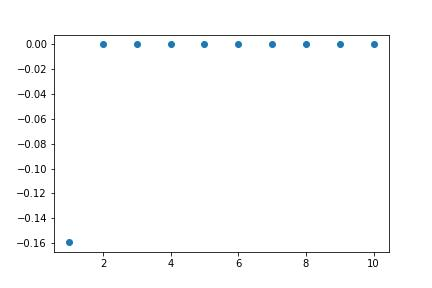
\includegraphics[width=0.9\textwidth, height=0.9\textwidth]{coefs_1_inv.jpg}
        \caption{Coefficients trouvés}
    \end{subfigure}
    \hfill
    \begin{subfigure}[b]{0.4\textwidth}
        \centering
        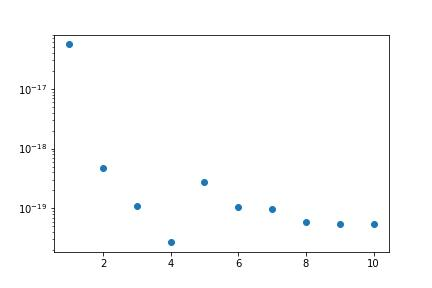
\includegraphics[width=0.9\textwidth, height=0.9\textwidth]{coefs_1_inv_erreur.jpg}
        \caption{Valeurs absolue de l'erreur pour chaque coefficient}
    \end{subfigure}
       \caption{Résultats de la méthode de l'inversion de système}
       \label{fig:résultats 1 inv}
\end{figure}



%%%%%%%%%%%%%%%%%%%%%%%%%%%%%%%%%%%%%%%%%%%%%%%%%%%%%%
\subsection{Algorithme de descente de gradients}

Profitons de cet exemple simple où le système est linéaire pour se familiariser avec l'algorithme de descente de gradients qui sera utile par la suite.
Le principe est de  partir d'un vecteur $\bm{A}^{(0)}$ choisit aléatoirement puis de calculer itérativement un nouveau vecteur $\bm{A}^{(k)}$ en se déplaçant dans l'espace dans la direction qui minimise le plus l'erreur localement.
On définit pour cela les paramètres suivants :

\begin{equation}
    \alpha>0, 
    \bm{A}^{(0)} = \begin{pmatrix}
                A_1^{(0)} \\
                A_2^{(0)} \\
                \vdots \\
                A_H^{(0)}
              \end{pmatrix},
    \bm{g}^{(0)} = \begin{pmatrix}
                \frac{\partial E^{(0)}}{\partial A_1^{(0)}} \\
                \frac{\partial E^{(0)}}{\partial A_2^{(0)}} \\
                \vdots \\
                \frac{\partial E^{(0)}}{\partial A_H^{(0)}}
              \end{pmatrix},     
\label{eq:définition descente de gradients}
\end{equation}

Puis on calcule itérativement :

\begin{equation}
    \bm{A}^{(k+1)} = \bm{A}^{(k)} - \alpha\bm{g}^{(k)} 
\label{eq:équation récurrence descente gradients}
\end{equation}

On cherche à trouver le coefficient $\alpha$ optimal qui assure la convergence tout en maximisant la vitesse de convergence.
On exprime tout d'abord le gradient en fonction de la matrice $\mathcal{M}$ et du vecteur $\bm{b}$ définis précédemment qui sont indépendants de $\bm{A}$ et de $k$:

\begin{equation}
    \bm{g}^{(k)} = \mathcal{M}\bm{A}^{(k)} - \bm{b}
\label{eq:expression matricielle gradient}
\end{equation}

Ainsi, l'équation de récurrence (\ref{eq:équation récurrence descente gradients}) se réécrit comme une suite arithmético-géométrique de vecteurs :

\begin{equation}
    \bm{A}^{(k+1)} = (\mathcal{I}_H - \alpha \mathcal{M} )  \bm{A}^{(k)} + \alpha\bm{b}
\label{eq:équation récurrence descente gradients v2}
\end{equation}

Cette équation de récurrence peut se réécrire si $\mathcal M$ est inversible en posant $\bm{A^*} = \mathcal {M}^{-1}\bm{b}$ (qui est l'unique solution du système linéaire) on arrive à l'expression de $\bm{A}^{(k)}-\bm{A^*} $ comme une suite géométrique :

\begin{equation}
    \begin{aligned}
        \bm{A}^{(k+1)}-\bm{A^*}  &= (\mathcal{I}_H - \alpha \mathcal{M} )  \bm{A}^{(k)} + \alpha\bm{b} - \mathcal {M}^{-1}\bm{b}\\
         &= (\mathcal{I}_H - \alpha \mathcal{M} ) (\bm{A}^{(k)}-\bm{A^*} )
    \end{aligned}
\label{eq:équation récurrence descente gradients v2}
\end{equation}

Pour s'assurer de la convergence de cette suite, on s'interresse au rayon spectral, c'est-à-dire le maximum du module des valeurs propres, de $\mathcal{R}_\alpha = (\mathcal{I}_H - \alpha \mathcal{M} )$, noté $\rho(\mathcal{R}_\alpha)$.
La suite $(\bm{A}^{(k)})_{k\in \mathbb{N}}$ converge si et seulement si la norme de $(\mathcal{R}_\alpha ^k)_{k\in \mathbb{N}}$ tend vers 0, sa limite est alors $\bm A^*$.
Cela est le cas si et seulement si $\rho(\mathcal{R}_\alpha)<1$ ~\cite{WikiRayonSpectral}.
De plus, elle convergera d'autant plus vite que son rayon spectral est faible.
On trace donc ce maximum en fonction de $\alpha$ en figure \ref{fig:choix alpha 1D}. 
On en déduit la valeur critique $\alpha_c = 6.2807.10^{-5}$, pour laquelle $\rho(\mathcal{R}_\alpha)=1$, ainsi que la valeur $\alpha_{min} = 6.2189.10^{-5}$ pour $\rho(\mathcal{R}_\alpha)$ est minimal.

On éxécute l'algorithme en parallèle pour les deux valeurs de $\alpha$ trouvées précédemment ainsi que pour une valeur $\alpha_1 = 6.3.10^{-5}$, tel que $\rho(\mathcal{R}_\alpha)>1$
On montre l'évolution de l'erreur en fonction du nombre d'itérations en figure \ref{fig:erreur selon alpha}. 
On constate que $\alpha_{min}$ donne lieu à une décroissance exponentielle de l'erreur pendant les 2000 premières itérations, qui 
devient ensuite stationnaire. 
Tandis que $\alpha_1$ donne une erreur qui croît exponentiellement car la norme de $(\mathcal{R}_\alpha ^n)_{n\in \mathbb{N}}$ diverge exponentiellement. 
La valeur $\alpha_c$ donne une erreur constante, 
elle correspond au cas limite entre les 2 cas précédents.

\begin{figure}
    \centering
    \begin{subfigure}[b]{0.4\textwidth}
        \centering
        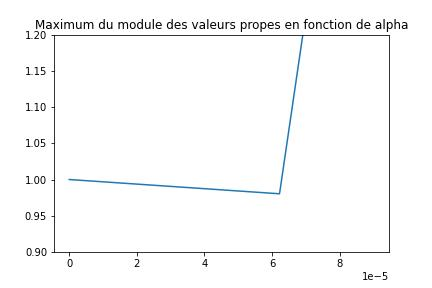
\includegraphics[width=0.8\textwidth, height=0.8\textwidth]{choix_alpha_1D.jpg}
        \caption{$\alpha \in [0, 10^{-4}]$}
    \end{subfigure}
    \hfill
    \begin{subfigure}[b]{0.4\textwidth}
        \centering
        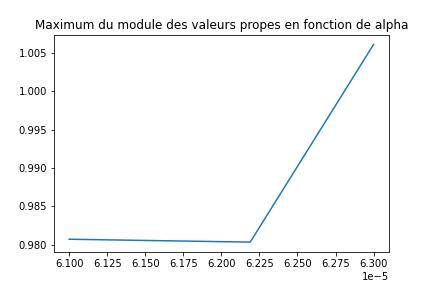
\includegraphics[width=0.8\textwidth, height=0.8\textwidth]{choix_alpha_1D_zoom.jpg}
        \caption{Au voisinage de l'intersection avec 1}
    \end{subfigure}
       \caption{Rayon spectral de $\mathcal{R}_\alpha$ en fonction de $\alpha$}
       \label{fig:choix alpha 1D}
\end{figure}


\begin{figure}
    \centering
    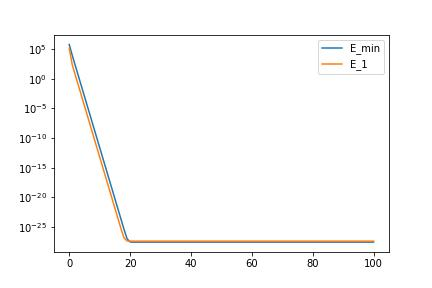
\includegraphics[width=0.8\textwidth]{comparaison_erreurs_selon_alpha_1D.jpg}
    \caption{Erreurs en fonction du nombre d'itérations pour 3 valeurs de $\alpha$}
    \label{fig:erreur selon alpha}
    \end{figure}


On retient donc les résultats obtenus pour $\alpha_{min}$ que l'on montre en figure \ref{fig:résultats 1 DG} avec les valeurs absolues des erreurs de chacun par rapport à la valeur théorique. 
On constate que les erreurs sur chaque coefficientest inférieure à $10^{-16}$, on valide donc cette seconde méthode.

Cette étude a mis en évidence l'importance du choix du taux d'apprentissage qui détermine le comportement de la suite de vecteurs obtenus lors de la descente de gradients. 
Cela sera important à garder en tête par la suite, même quand les systèmes à résoudre ne seront plus linéaire et qu'il ne sera plus possible de déterminer à l'avance les valeurs optimales. 
Elles devront donc être testées empiriquement.


\begin{figure}
    \centering
    \begin{subfigure}[b]{0.4\textwidth}
        \centering
        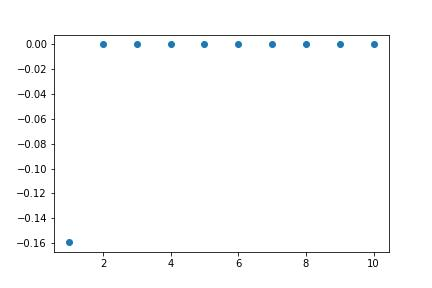
\includegraphics[width=0.9\textwidth, height=0.9\textwidth]{coefs_1_DG.jpg}
        \caption{Coefficients trouvés}
    \end{subfigure}
    \hfill
    \begin{subfigure}[b]{0.4\textwidth}
        \centering
        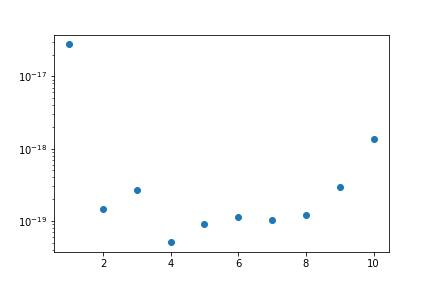
\includegraphics[width=0.9\textwidth, height=0.9\textwidth]{coefs_1_DG_erreur.jpg}
        \caption{Valeurs absolue de l'erreur pour chaque coefficient}
    \end{subfigure}
       \caption{Résultats de la méthode de descnte de gradients}
       \label{fig:résultats 1 DG}
\end{figure}



%%%%%%%%%%%%%%%%%%%%%%%%%%%%%%%%%%%%%%%%%%%%%%%%%%%%%%%%%%%%%%%%%%%%
\section{Solutions par réseau de neurones}

On cherche à présent à utiliser un réseau de neurones pour approcher la solution de l'équation différentielle. On cherche désormais des solutions approchées sous la forme suivante :

\begin{equation}
\left\{
    \begin{aligned}
        \Tilde{M}(t) &= M_0 + t{\mathcal{N}}(t,\bm{P}) \\
        {\mathcal{N}}(t,\bm{P}) &= \sum_{j=1}^{H} v_j \sigma(w_jt+b_j)
    \end{aligned}
\right.
\label{eq:solution NN}
\end{equation}

${\mathcal{N}}(t,\bm{P})$ correspond donc à la sortie d'un réseau de neurones dont l'architecture est présentée en figure \ref{fig:NN}, contenant une couche cachée intermédiaire, qui réalise en sortie une somme pondérée de sigmoïdes, la fonction utilisée est ${\displaystyle{\forall x \in \mathbf{R}, \sigma(x) = \frac{1}{1+e^{-x}}}}$. Les paramètres $\bm{P}$ à ajuster sont désormais les coefficients $(w_j)_{j\in \llbracket 1,H \rrbracket}$, $(b_j)_{j\in \llbracket 1,H \rrbracket}$ et $(v_j)_{j\in \llbracket 1,H \rrbracket}$.

{\color{red}Peux-tu donner une référence pour quelqu'un qui cherche ce que tout ceci veut dire?}
\begin{figure}
\centering
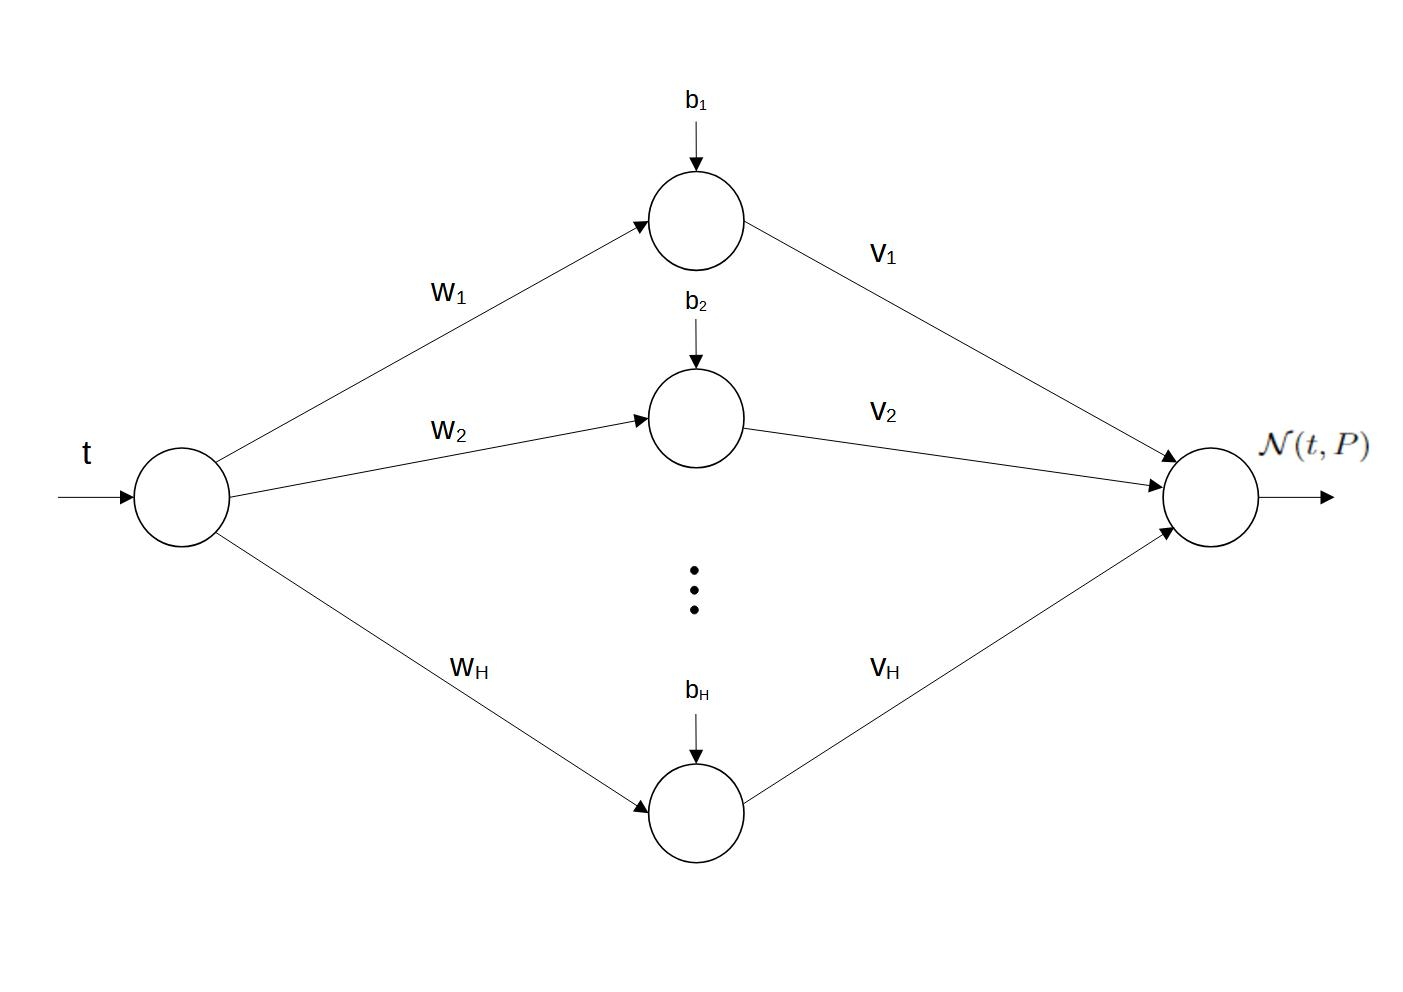
\includegraphics[width=0.8\textwidth]{NN.jpg}
\caption{\label{fig:NN}Réseau de neurones}
\end{figure}

On définit une nouvelle fonction d'erreur, calculée à partir des $N$ points suivants : $\forall i \in\llbracket 1,N \rrbracket, t_i = \frac{i-1}{N-1} $ 

\begin{equation}
        E(\bm{P}) = \sum_{i=1}^{N} (\frac{d\Tilde{M}}{dt}(t_i) + \cos(2\pi t_i))^2
\label{eq:erreur NN}
\end{equation}


On calcule ensuite les expressions analytiques des dérivées partielles de $E(\bm{P})$ par rapport à chaque paramètre ajustable, puis on cherche à minimiser cette erreur à l'aide de l'algorithme de descente de gradients.

%%%%%%%%%%%%%%%%%%%%%%%%%%%%%%%%%%%%%%%%%%%%%%%%%%%%%%
\subsection{Résultats obtenus}
On initialise l'algorithme avec les paramètres suivants : $(H=4, N=20)$
On obtient une erreur de $1,2.10^{-2}$ et une estimation visible en figure \ref{fig:resultat_NN}. Cela permet de valider notre modèle sur l'étude à une dimension.

\begin{figure}
\centering
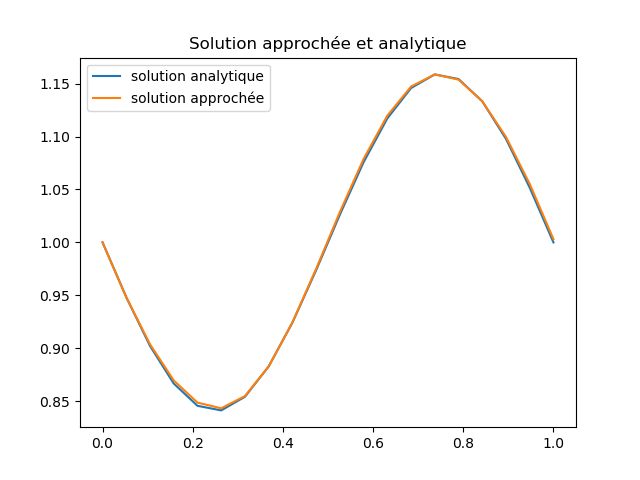
\includegraphics[width=0.8\textwidth]{resultat_NN.png}
\caption{\label{fig:resultat_NN}estimation de la solution par un réseau de neurones}
\end{figure}

%%%%%%%%%%%%%%%%%%%%%%%%%%%%%%%%%%%%%%%%%%%%%%%%%%%%%%
\chapter{Mouvement de précession}
\label{chap:precession}
On s'intéresse désormais à l'équation de la précession de Larmor~\cite{PrecessionLarmor} pour un moment magnétique $\bm{M} \in \mathbb{R}^3$ autour d'un vecteur ${\bm{\omega}}$ pointant le long de l'axe $z$ et dont la composante sur cet axe est constante, soit $\bm{\omega}=\omega_z{\bm z}$.

\begin{equation}
    \frac{d\bm{M}}{dt} = \bm{\omega}\times\bm{M} 
    \label{eq:equation Larmor}
\end{equation}

Cette équation implique que $\frac{d\bm{M}}{dt} $ et $\bm{\omega}$ soient orthogonaux, ainsi $\frac{dM_z}{dt}=0$. Par conséquent, on ne considérera que les composantes selon les vecteurs $\bm{x}$ et $\bm{y}$ et l'équation~\ref{eq:equation Larmor} se réécrit ainsi comme un système de deux équations différentielles couplées : 

\begin{equation}
\left\{
    \begin{aligned}
        \frac{dM_x}{dt} &= \omega M_y \\
        \frac{dM_y}{dt} &= -\omega M_x
    \end{aligned}
\right.
\end{equation}

On cherchera les solutions pour $t\in [t_a=0,t_b=1]$, en imposant les conditions initiales suivantes :
\begin{equation}
\left\{
    \begin{aligned}
        M_x(0) &= M_0 \\
        M_y(0) &= 0
    \end{aligned}
\right.
\label{eq:équations couplées}
\end{equation}

On pourra ensuite comparer nos résultats avec la solution analytique connue de ce système qui vaut :

\begin{equation}
\left\{
    \begin{aligned}
        M_x(t) &=  M_0 \cos(2\omega t)\\
        M_y(t) &= -M_0 \sin(2\omega t)
    \end{aligned}
\right.
\label{eq:solution analytique couplée}
\end{equation}

\section{Solutions en séries de Fourier}
On cherche des solutions numériques approchées sous la forme de séries de Fourier tronquées avec $H$ harmoniques, en posant la forme suivante :

\begin{equation}
\left\{
    \begin{aligned}
        \Tilde{M}_x(t) &= M_0 + \sum_{m=1}^{H} A_m (\cos(m\omega t)-1) + B_m \sin(m\omega t) \\
        \Tilde{M}_y(t) &= \sum_{m=1}^{H} -A_m \sin(m\omega t) + B_m (\cos(m\omega t)-1)
    \end{aligned}
\right.
\label{eq:solution Fourier couplée}
\end{equation}

Les coefficients $(A_m)_{m\in \llbracket 1,H \rrbracket}$ et $(B_m)_{m\in \llbracket 1,H \rrbracket}$ sont les paramètres à ajuster.
On cherche à obtenir la solution analytique, i.e $\forall m \in\llbracket 1,H \rrbracket, A_m = \delta _1 ^m $ et $\forall m \in\llbracket 1,H \rrbracket, B_m = 0 $. 

On définit une fonction d'erreur pour ces solutions potentielles, en s'interressant aux $N$ points suivants : $\forall i \in\llbracket 1,N \rrbracket, t_i = \frac{i-1}{N} $ :

\begin{equation}
        E(\bm{P}) = \sum_{i=1}^{N} (\frac{d\Tilde{M}_x}{dt}(t_i) - \omega \Tilde{M}_y(t_i))^2 + (\frac{d\Tilde{M}_y}{dt}(t_i) + \omega \Tilde{M}_x(t_i))^2
\label{eq:erreur descente gradient couplées}
\end{equation}

On utilise ensuite la méthode de descente de gradients définie précédemment, en calculant les dérivées partielles suivantes :
$(\frac{\partial E}{\partial A_l}, \frac{\partial E}{\partial B_l})_{l \in \llbracket 1,H \rrbracket}$

On peut se ramener à l'écriture du cas à une dimension définissant le vecteur $\bm{P}$ comme la concaténation des vecteurs $\bm{A}$ et $\bm{B}$ et le vecteur $\bm{g}$ comme le vecteur contenant les dérivées  partielles de $E$ par rapport à chaque composante de $\bm{P}$. 

\begin{equation}
    \bm{P}^{(k)} = \begin{pmatrix}
                A_1^{(k)} \\
                \vdots \\
                A_H^{(k)} \\
                B_1^{(k)} \\
                \vdots \\
                B_H^{(k)}
              \end{pmatrix},
    \bm{g}^{(k)} = \begin{pmatrix}
                \frac{\partial E^{(k)}}{\partial A_1^{(k)}} \\
                \vdots \\
                \frac{\partial E^{(k)}}{\partial A_H^{(k)}} \\
                \frac{\partial E^{(k)}}{\partial B_1^{(k)}} \\
                \vdots \\
                \frac{\partial E^{(k)}}{\partial B_H^{(k)}} 
              \end{pmatrix},     
\label{eq:définition descente de gradients 2D}
\end{equation}

Il existe alors une nouvelle matrice $\mathcal{M}$ d'ordre $2H$ ainsi qu'un nouveau vecteur $\bm{b}$ de taille $2H$ tels que les équations définissant la descente de gradients soient les suivantes :

\begin{equation}
    \bm{P}^{(k+1)} = \bm{P}^{(k)} - \alpha\bm{g}^{(k)} 
\label{eq:équation récurrence descente gradients 2D}
\end{equation}

\begin{equation}
    \bm{g}^{(k)} = \mathcal{M}\bm{P}^{(k)} - \bm{b}
\label{eq:expression matricielle gradient 2D}
\end{equation}

\begin{equation}
    \bm{P}^{(k+1)} = (\mathcal{I}_H - \alpha \mathcal{M} )  \bm{P}^{(k)} + \alpha\bm{b}
\label{eq:équation récurrence descente gradients v2 2D}
\end{equation}

On réalise la même étude qu'en dimension 1 pour la recherche du coefficient $\alpha_{min}$ qui minimise le maximum des modules des valeurs propres de $\mathcal{R}_\alpha = \mathcal{I}_H - \alpha \mathcal{M}$, ainsi que le coefficient $\alpha_c$ à ne pas dépasser, à partir duquel ce maximum et supérieur à 1 et la suite diverge.
On trouve les valeurs suivantes $\alpha_{min} = 6.0906.10^{-6}$ et $\alpha_c = 6.1146.10^{-6}$,  et l'évolution du maximum en fonction de $\alpha$ est montré en figure \ref{fig:choix_alpha_2D}.


\begin{figure}
    \centering
    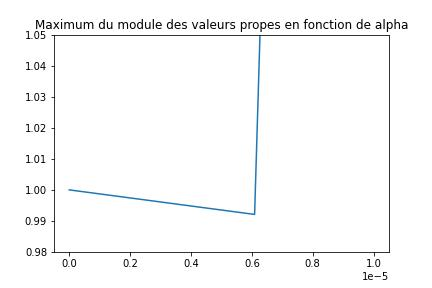
\includegraphics[width=0.7\textwidth]{choix_alpha_2D.jpg}
    \caption{\label{fig:choix_alpha_2D}Evolution du maximum du module en fonction de $\alpha$}
\end{figure}

On éxécute l'algorithme en choisissant la valeur $\alpha_{min}$ précédente et on montre l'évolution de l'erreur en fonction du nombre d'itérations en figure \ref{fig:Erreur_2_DG}. 
On constate comme dans le cas à 1 dimension que $\alpha_{min}$ donne lieu à une décroissance exponentielle de l'erreur, cette fois pendant les 4500 premières itérations, qui devient ensuite quasiment stationnaire, de l'ordre de $10^{-25}$.

\begin{figure}
    \centering
    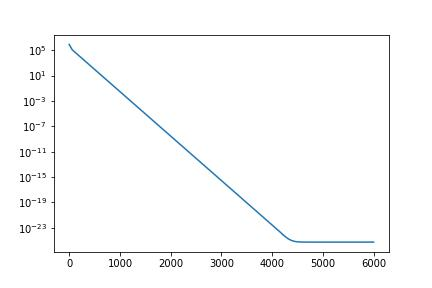
\includegraphics[width=0.7\textwidth]{Erreur_2_DG.jpg}
    \caption{\label{fig:Erreur_2_DG}Valeur de la fonction d'erreur en fonction du nombre d'itérations}
\end{figure}

Les coefficients finaux de $\bm{P}$ ainsi que les valeurs absolues de leurs erreurs sont représentées en figure \ref{fig:résultats 2 DG}.
On peut constater que l'on retrouve bien les coefficients attendus, avec une erreur au maximum de l'ordre de $10^{-15}$.

\begin{figure}
    \centering
    \begin{subfigure}[b]{0.4\textwidth}
        \centering
        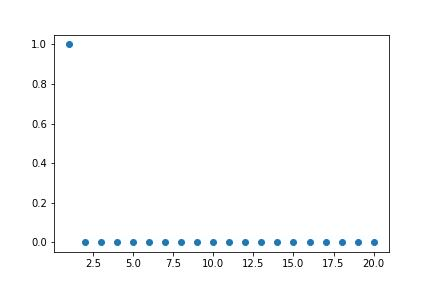
\includegraphics[width=0.9\textwidth, height=0.9\textwidth]{coefs_2_DG.jpg}
        \caption{Coefficients trouvés}
    \end{subfigure}
    \hfill
    \begin{subfigure}[b]{0.4\textwidth}
        \centering
        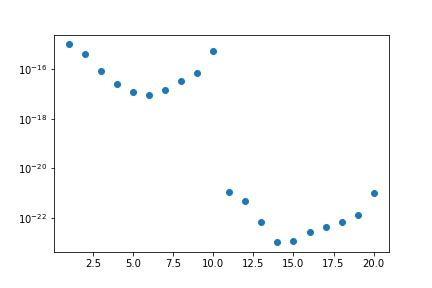
\includegraphics[width=0.9\textwidth, height=0.9\textwidth]{coefs_2_DG_erreur.jpg}
        \caption{Valeurs absolue de l'erreur pour chaque coefficient}
    \end{subfigure}
       \caption{Résultats de la méthode de descente de gradients pour le mouvement de précession}
       \label{fig:résultats 2 DG}
\end{figure}

\section{Solutions aprochées par un réseau de neurones}

On cherche dans ce paragraphe à approcher la solution du système des 2 équations grâce à un réseau de neurones.
On choisit l'architecture suivante pour le réseau de neurones : 
1 entrée pour la variable temporelle, une première couche intermédiaire de $h_1=32$ neurones, une seconde couche intermédiaire de $h_2=8$ neurones, toutes deux utilisant la sigmoïde définie précédement comme fonction d'activation, et enfin 2 neurones de sortie connectées à la deuxième couche intermédiaire, avec l'identité comme fonction d'activation en sortie.
On note les sorties de ces deux derniers neurones respectivement $\mathcal{N}_x(t, \bm{P})$ et $\mathcal{N}_y(t, \bm{P})$, où $\bm{P}$ représente l'ensemble des paramètres du réseau de neurones.
On construit alors nos solutions approchées de la façon suivante :

\begin{equation}
    \left\{
        \begin{aligned}
            \Tilde{M}_x(t) &= M_0+ t\mathcal{N}_x(t, \bm{P}) \\
            \Tilde{M}_y(t) &= t\mathcal{N}_y(t, \bm{P})
        \end{aligned}
    \right.
    \label{eq:solution 2_NN}
    \end{equation}

On définit une fonction d'erreur pour ces solutions potentielles, en s'interressant aux $N$ points suivants de l'intervalle $[t_a=-1, t_b=1]$: 
$\forall i \in\llbracket 1,N \rrbracket, t_i = -1 + 2\frac{i-1}{N} $ :

\begin{equation}
        E(\bm{P}) = \frac{1}{N}\sum_{i=1}^{N} (\frac{d\Tilde{M}_x}{dt}(t_i) - \omega \Tilde{M}_y(t_i))^2 + (\frac{d\Tilde{M}_y}{dt}(t_i) + \omega \Tilde{M}_x(t_i))^2
\label{eq:erreur 2_NN}
\end{equation}


On choisit ensuite les paramètres d'entraînement suivants : taux d'apprentissage : 0.007,50000 itérations, et on lance 3 entraînements pour $N \in \{10,40,100\}$. 
On obtient les résultats montrés en figure \ref{fig:résultats 2 NN en fonction de N}, où l'axe vertical représente le temps, et les axes horizontaux représentent $M_x$ et $M_y$. 
La solution analytique est représentée en orange, la solution approchée est représentée en bleu, et les points rouges sont les points correspondant aux points d'entraînement $(t_i)_{i \in \llbracket 1, N \rrbracket}$.


\begin{figure}
    \centering
    \begin{subfigure}[b]{0.4\textwidth}
        \centering
        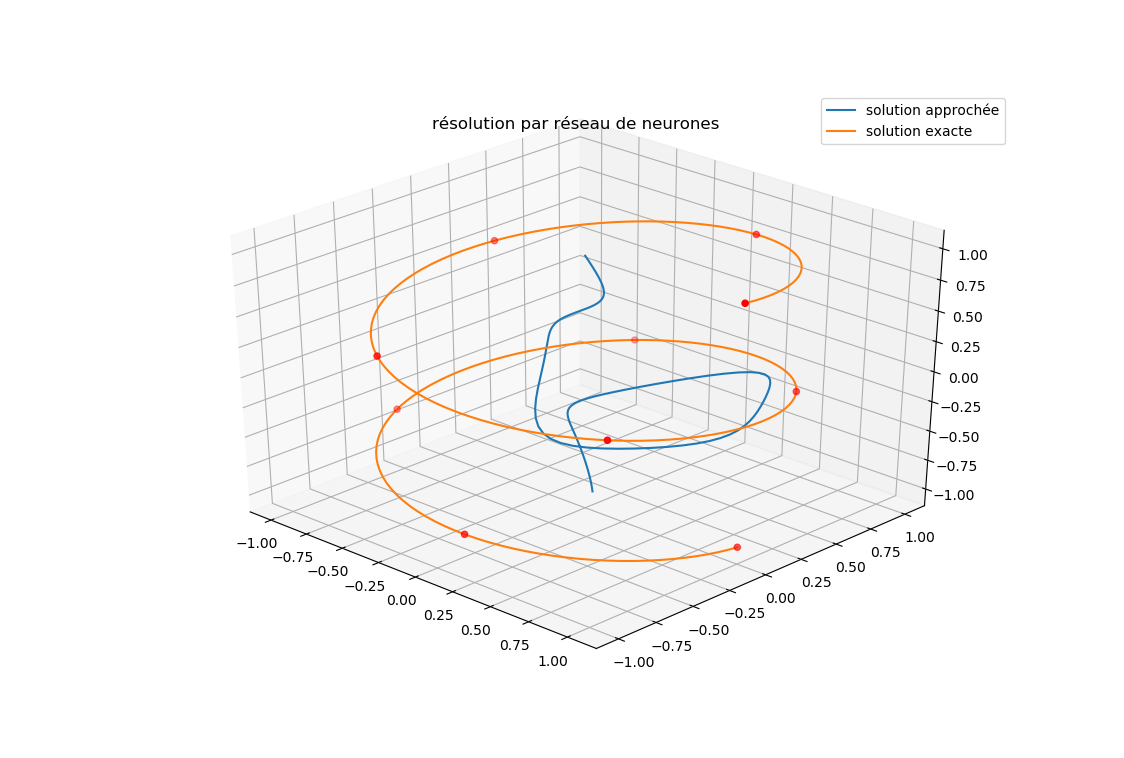
\includegraphics[width=1\textwidth, height=0.9\textwidth]{direct_training_N=10.png}
        \caption{Solution obtenue pour $N=10$}
    \end{subfigure}
    \hfill
    \begin{subfigure}[b]{0.4\textwidth}
        \centering
        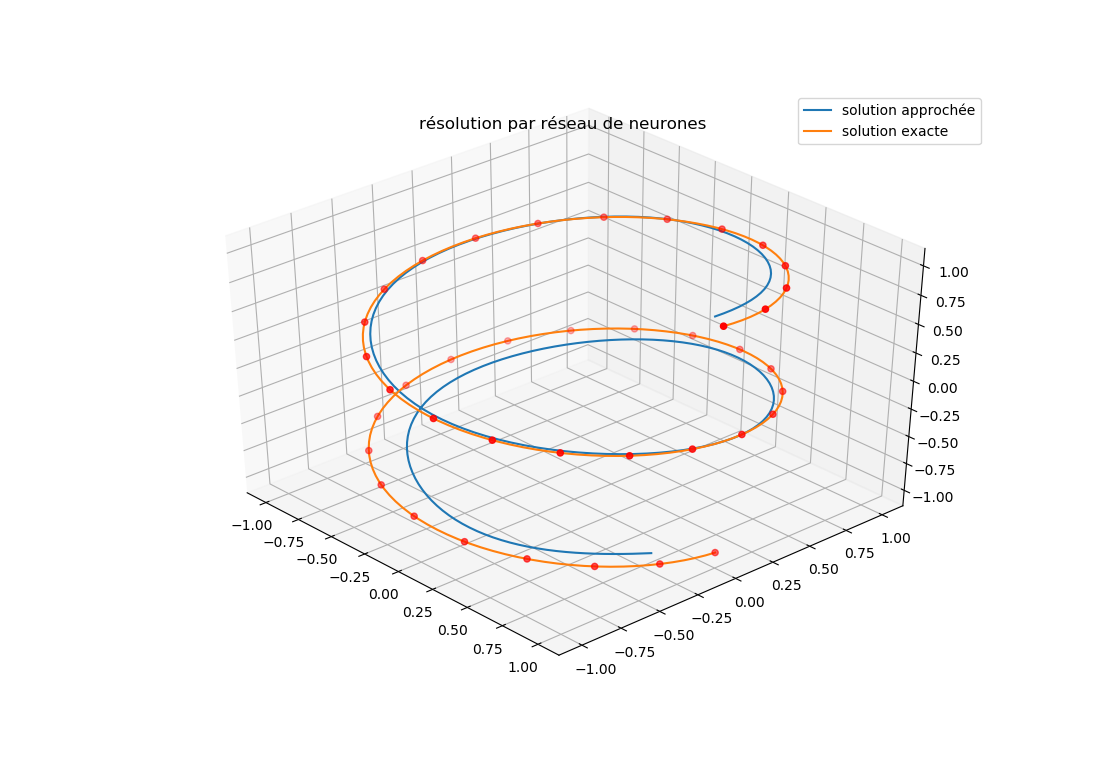
\includegraphics[width=1\textwidth, height=0.9\textwidth]{direct_training_N=40.png}
        \caption{Solution obtenue pour $N=40$}
    \end{subfigure}
    \hfill
    \begin{subfigure}[b]{0.4\textwidth}
        \centering
        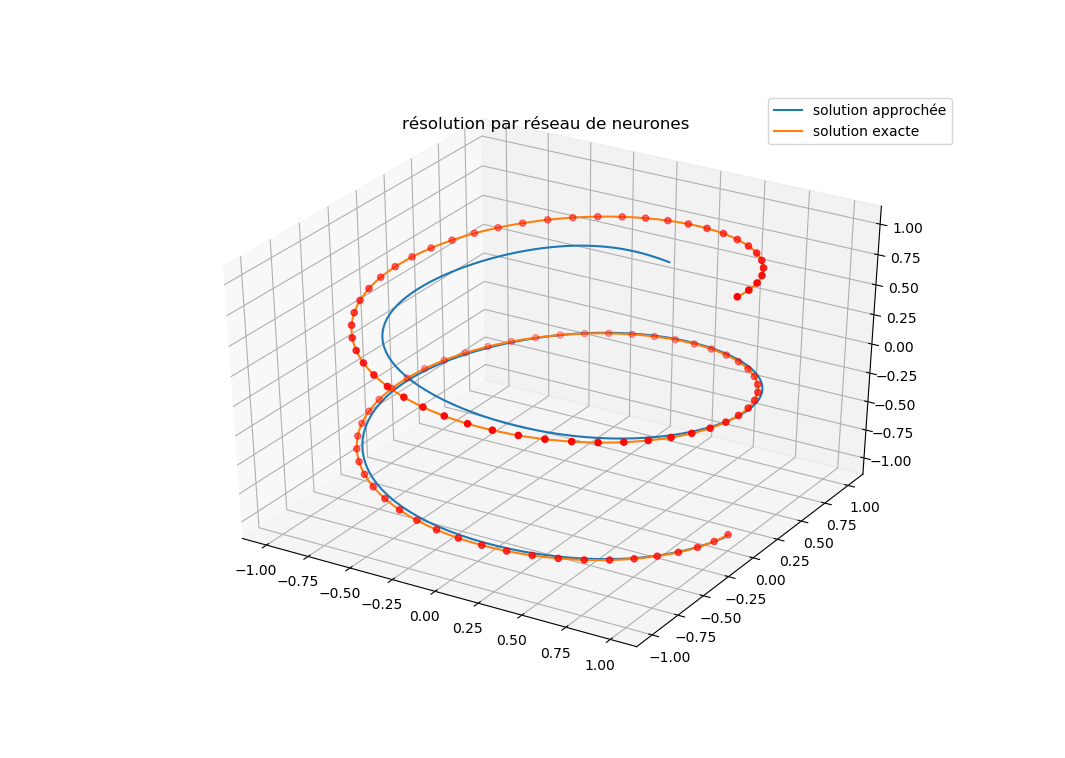
\includegraphics[width=1\textwidth, height=0.9\textwidth]{direct_training_N=100.png}
        \caption{Solution obtenue pour $N=100$}
    \end{subfigure}
       \caption{Représentations graphiques de $M_x$ et  $M_y$ en fonction du temps par le réseau de neurones}
       \label{fig:résultats 2 NN en fonction de N}
\end{figure}


%%%%%%%%%%%%%%%%%%%%%%%%%%%%%%%%%%%%%%%%%%%%%%%%%%%%%%%%%%%%%%
\chapter{Précession avec amortissement}
\label{chap:precession_gilbert}

Dans ce chapitre, on s'intéresse à déterminer le mouvement de précession d'un moment magnétique $\bm{M} \in \mathbb{R}^3$ amorti.
Son équation d'évolution est représentée en fonction d'une constante d'amortissement réelle et sans dimension notée $\lambda$ et s'établit, pour simplifier, autour d'un vecteur ${\bm{\omega}}$ pointant le long de l'axe $z$ et dont la composante sur cet axe est constante, soit $\bm{\omega}=\omega_z{\bm z}$.

L'équation considérée prend le nom d'équation de precession avec un terme d'amortissement introduit par Gilbert~\cite{EquationGilbert} et s'écrit

\begin{equation}
    \frac{d\bm{M}}{dt} = (\bm{\omega}-\lambda \frac{d{\bm{M}}}{dt})\times\bm{M} 
    \label{eq:equation Gilbert}
\end{equation}

Cette équation vectorielle admet plusieures propriétés remarquables que nous allons exploiter.

%%%%%%%%%%%%%%%%%%%%%%%%%%%%%%%%%%%%%%%%%%%%%%%%%%%%%%%%%%%%%%%%
\section{Projection en coordonnées cartésiennes}
\label{sec:projection_cartesiennes}

En prenant le produit vectoriel par $\bm M$ à gauche des deux membres de l'équation~\ref{eq:equation Gilbert}, on forme une projection sur un plan normal à $\bm{M}$, et on obtient 3 nouvelles équations différentielles scalaires (après un chagement d'échelle temporelle) :
\begin{equation}
    \left\{
        \begin{aligned}
            \frac{dM_x}{d\tilde{t}} &= - M_y\omega_z - \lambda M_x M_z \omega_z \\
            \frac{dM_y}{d\tilde{t}} &= M_x\omega_z - \lambda M_y M_z \omega_z \\
            \frac{dM_z}{d\tilde{t}} &= \lambda\omega_z (1-M_z^2) 
        \end{aligned} 
    \right. 
    \label{eq:equations scalaires Gilbert}
\end{equation}

On remarque que l'équation sur $M_z$ est découplée des 2 autres, on cherche ainsi à résoudre celle-ci en premier lieu.

%%%%%%%%%%%%%%%%%%%%%%%%%%%%%%%%%%%%%%%%%%%%%%%%%%%%%%%%
\subsection{Résolution de l'équation sur $M_z$}


On utilise la même approche avec un réseau de neurones que précédemment à l'aide d'un réseau de neurones.
On réalisera à présent les implémentations en python à l'aide de la bibliothèque TensorFlow.

On choisit comme architecture du réseau de neurones une entrée pour la variable temporelle, suivie de couches intermédiaires contenant respectivement $h_1$ et $h_2$ neurones, connectés à la sortie unique du réseau de neurones, dont les paramètres sont représenté par le vecteur $\bm{P}$.
Comme précédemment, afin de satisfaire la condition initiale, on cherche les fonction $\tilde{M_z}$ sous la forme suivante, où ${\mathcal{N}}(\Tilde{t},\bm{P})$ représente la sortie du réseau de neurones.

\begin{equation}
    \Tilde{M_z}(\Tilde{t}) = M_z(0) +\Tilde{t} {\mathcal{N}}(\Tilde{t},\bm{P}) 
    \label{eq:solution NN Mz}
\end{equation}

On définit la fonction d'erreur suivante :


On fixe les paramètres suivants : $\lambda = 0.3$, nombre de points de tests : $N=30$, 
intervalle d'étude : $[t_a = -1, t_b = 1]$, $M_z(0) = 0$.
Lors des essais d'entraînement du modèle on fait face à plusieurs problèmes.
On remarque que souvent la sortie du réseau de neurones est quasiment constantesur l'intervalle d'étude. 
Ainsi, il semble que l'entraînement ne consiste alors dans ce cas qu'à ajuster cette valeur constante pour minimser la fonction d'erreur dans le cas où $M_z$ est linéaire par rapport à $\tilde{t}$, (d'après l'équation \ref{eq:solution NN Mz},pour ${\mathcal{N}}(\Tilde{t},\bm{P}) = \mu\in \mathbf{R}$ constante, et $M_z(0) = 0$).

Après plusieurs essais d'entraînement, on remarque que l'on tombe sur l'une ou l'autre des 2 solutions présentées en figure \ref{fig:minimums locaux Mz}.

\begin{figure}
    \centering
    \begin{subfigure}[b]{0.4\textwidth}
        \centering
        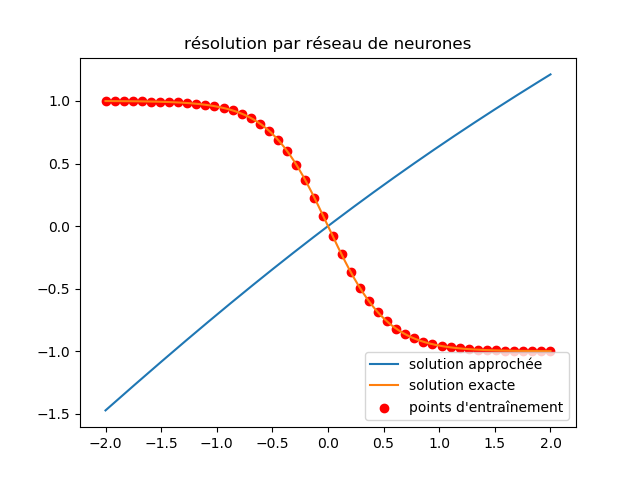
\includegraphics[width=0.9\textwidth, height=0.9\textwidth]{min_loc1.png}
        \caption{Première solution linéaire}
    \end{subfigure}
    \hfill
    \begin{subfigure}[b]{0.4\textwidth}
        \centering
        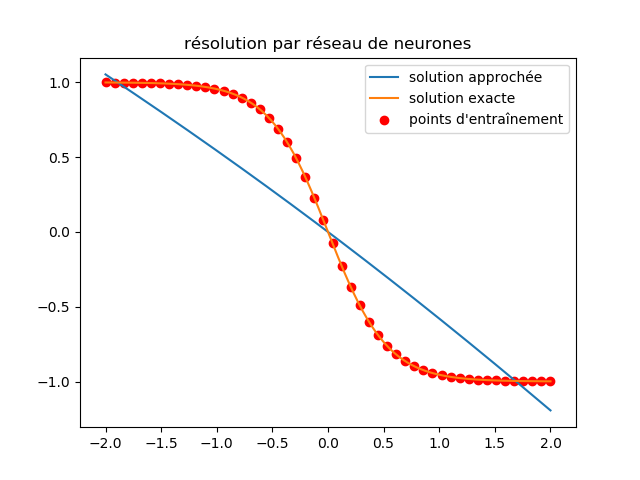
\includegraphics[width=0.9\textwidth, height=0.9\textwidth]{min_loc2.png}
        \caption{Seconde solution linéaire}
    \end{subfigure}
       \caption{Solutions trouvées pour $M_z$ après de rapides entraînements}
       \label{fig:minimums locaux Mz}
\end{figure}

On peut vérifier cette hypothèse en exprimant analytiquement notre fonction d'erreur pour une fonction $M_z$ linéaire : $\forall \tilde{t} \in \mathbf{R}, \tilde{M_z}(\tilde{t}) = \mu  \tilde{t}$. 
On peut calculer notre erreur, en fonction de $\mu$, en remplaçant la somme discrète par une intégrale qui peut être calculée facilement car 
l'intégrande est alors une fonction polynomiale en $\tilde{t}$ :

\begin{equation}
    \begin{aligned}
        E(\mu) &= \frac{1}{t_b-t_a}\int_{t_b}^{t_a} (\frac{d\tilde{M_z}}{d\tilde{t}}(\tilde{t})-\lambda \omega_z (\tilde{M_z}(t)^2-1))^2 \,d \tilde{t} \\
        E(\mu) &= \frac{16}{5}\lambda^2\omega_z^2\mu^4 
            - \frac{8}{3}\lambda\omega_z\mu^3
            + (1- \frac{8}{3}\lambda^2\omega_z^2)\mu^2
            + 2\lambda\omega_z\mu
            + \lambda^2\omega_z^2
    \end{aligned}
    \label{eq:fonction d'erreur analytique, M_z linéaire}
\end{equation}

On remarque alors que cette fonction admet deux minimums locaux qui ont pour valeurs approchées : $ \mu_a \approx 0.696$, $E(\mu_a) \approx 3.04$ et $\mu_b \approx -0.574$,$ E(\mu_b) \approx -0.78$. 
Cela est effectivement proche des valeurs que l'on obtient lors des entraînements montrés en figure \ref{fig:minimums locaux Mz}.
En effet, sur le premier exemple, la sortie du réseau de neurones varie entre 0.60 et 0.74 sur l'intervalle étudié, et la valeur finale de l'erreur est 3.04, ce qui correspond à $\mu_b$ et $E(\mu_b)$.
Pour le second exemple, la sortie est comprise entre -0.60 et -0.52, et l'erreur vaut 0.82, ce qui correspond bien au second minimum local $E(\mu_a)$.

On peut alors remettre en question le modèle choisi pour notre réseau de neurones, qui n'est pas forcément le plus adapté. 
On peut par exemple essayer de changer les fonctions d'activation utilisées par les couches intermédiaires, qui étaient des sigmoïdes, et les remplacer par la fonction $relu$.

On a ainsi pu obtenir des résultats satisfaisants visibles en figure \ref{fig:relu apprentissage direct} en lançant l'entraînement avec les fonctions $relu$ pour 10000 itérations, avec un taux d'apprentissage de $10^{-3}$,$N=50$, $[t_a = -1, t_b = 1]$.
L'erreur finale est de 0.018.

Ainsi, la fonction $relu$ semble faciliter la convergence du réseau de neurones.

\begin{figure}
    \centering
    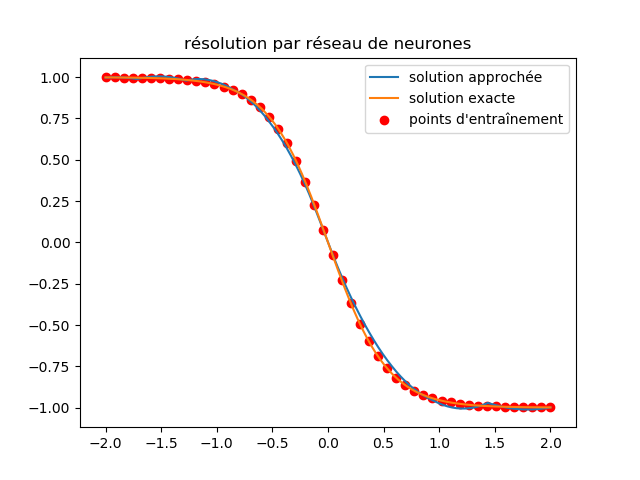
\includegraphics[width=0.8\textwidth]{direct_relu_0.001_10000_32_16_v2.png}
    \caption{Résultats obtenus avec la fonction d'activation $relu$}
    \label{fig:relu apprentissage direct}
\end{figure}

\subsection{Résolution des équations sur Mx et My}

%%%%%%%%%%%%%%%%%%%%%%%%%%%%%%%%%%%%%%%%%%%%%%%%%%%%%%%%%%%%%%%%%%%%%%%%%%%%%%
\chapter{Conclusion et perspectives}
\label{Conclusion}

\begin{thebibliography}{2}
    \bibitem{EquationGilbert}{\href{https://fr.wikipedia.org/wiki/%C3%89quation_de_Landau-Lifshitz-Gilbert}{Wikipedia, Équation de Landau-Lifshitz-Gilbert
    }}
    \bibitem{PrecessionLarmor}{\href{https://fr.wikipedia.org/wiki/Pr%C3%A9cession_de_Larmor}{Wikipedia, Précession de Larmor
    }}
    \bibitem{MLWithApp}{\href{https://doi.org/10.1016/j.mlwa.2021.100058}{T.T.Dufera, Machine Learning With Applications {\bf5} 100058 (2021)}}
    \bibitem{ANNforOPDEs}{\href{https://doi.org/10.1109/72.712178}{I. E. Lagaris, A. Likas and D. I. Fotiadis, IEEE Transactions on Neural Networks {\bf9} no. 5 pp. 987-1000 (1998)}}
    \bibitem{HighOrderHybrid}{\href{https://doi.org/10.1016/j.amc.2006.05.068}{A.Malek * and R.Shekari Beidokhti, Applied Mathematics and Computation {\bf183} 260–271(2006)}}
    \bibitem{FunctionApproximation}{\href{https://dl.acm.org/doi/10.5555/1466915.1466916#}{Z.Zainuddin and P.Ong, WSEAS Transactions on Mathematics Volume {\bf7} Issue 6 pp 333–338(2008)}}
    \bibitem{WikiNN}{\href{https://en.wikipedia.org/wiki/Artificial_neural_network}{Wikipedia, Réseaux de neurones
    }}
    \bibitem{WikiRayonSpectral}{\href{https://en.wikipedia.org/wiki/Spectral_radius#Power_sequence}{Wikipedia, Rayon spectral et suites des puissances
    }}
    
\end{thebibliography}


\end{document}

